\chapter{Preparatory Work}\label{ch:samples}
%{\raggedleft ``\emph{Il dolce non lo mangi mai, ma qualche volta ti rifai.} \par}
%{\raggedleft \emph{Abbracciami}"\par}
%{\raggedleft -- Pietro Ciampi, L'amore e' tutto qui, 1971 -- \par}
%\vspace{0.5cm}

%{\raggedleft ``\emph{You never eat dessert, but, sometimes, you make up for it.} \par}
%{\raggedleft \emph{Hug me}"\par}
%{\raggedleft -- Pietro Ciampi, L'amore e' tutto qui, 1971 -- \par}
%\vspace{0.5cm}


This chapter describes the preparatory work done on the the data and Monte Carlo samples used for the cross section analyses. 
This entails the choice of the data set and the production of the information needed to construct the Monte Carlo Simulation~(section \ref{sec:dataSet}),  the construction and use of said Monte Carlo simulation~(section \ref{sec:MCSet}), the study and optimization of the tracking in the TPC for the cross section analyses~(section \ref{sec:TrackingStudies}),  the calibration of the calorimetry response and related energy studies~(section \ref{ch:energyCal}). 



\section{Cross Section Analyses Data Set}\label{sec:dataSet}
We choose LArIAT Run-II as the data period for the  ($\pi^{-}$,Ar) and (K$^{+}$,Ar) total hadronic cross section analyses. 
Data taking for the this period started on 03/15/2016  and ended on 07/31/2016. 
Since we are interested in beamline and TPC information, we ask basic requirements on the operational status of the time of fight, wire chambers and TPC to form the good run list for this period, which we informally call ``lovely runs".

The subset of lovely runs  chosen for the  ($\pi^{-}$,Ar) total hadronic cross section analysis includes only the -60A and -100A magnet configurations in negative polarity, even if LArIAT explored several other beamline configurations during Run-II. The -60A and -100A combined data set accounts for approximately 90\% of the total Run-II negative polarity runs.   Since the production of beamline Monte Carlo depends on the wanted beamline configuration, the choice of only two beamline settings limits the need for beamline MC production. 

Similarly, the subset of lovely runs chosen  for the (K$^{+}$,Ar)  total hadronic cross section analysis includes only the +60A and +100A magnet configurations in positive polarity. It should be noted that kaons are extremely rare in the +60A sample, thus the data sample for the (K$^{+}$,Ar) cross section after the mass selection is about 90\% +100A runs, as shown in Table \ref{tab:databreakdown}.

For the first measurements in LArIAT that uses both beamline and TPC information, we choose strict requirements on the reconstruction of the WC tracks, the so-called ``Picky Track" sample (see \ref{sec:MWPCfunc}). This choice presents two advantages:  the uncertainty on the momentum reconstruction for the ``Picky Tracks" sample is smaller compared to the ``High Yield" sample, and the comparison with the beamline MC results is straightforward. A possible future update and cross check of these analysis would be the use of the High Yield sample, where the statistics is about three times higher. 

The breakdown of beamline events as a function of the magnets settings is shown in Table \ref{tab:databreakdown}. 
The choice of the data sets determines the production of beamline MC and serves as basis for the production of Data Driven MC, as shown in the next sections.

\begin{table}[b]
\centering
\begin{tabular}{|l|c|c|c|}  
\hline
                                                              & I = 60 A          & I = 100 A   & Total     \\ \hline
Data Events after $\pi/\mu/e$ Mass Selection     &     67068          &  71413  & 138481 \\ \hline
Data Events after $K$ Mass Selection                &     274              &   2563   & 2837  \\ \hline
\end{tabular}
\caption{Number of data events which fit the $\pi/\mu/e$ or $K$ mass hypothesis as a function of magnet settings.}
\label{tab:databreakdown}
\end{table}



\section{Construction of a Monte Carlo Simulation for LArIAT}\label{sec:MCSet}
For the simulation of LArIAT events and their particle make up, we use a combination of two MC generators: the G4Beamline Monte Carlo and the Data Driven single particle Monte Carlo (DDMC). We use the G4Beamline MC to simulate the particle transportation in the beamline and calculate the particle composition of the beam just after the fourth Wire Chamber (WC4). In order to simulate the beamline particles after WC4 and in the TPC, we use the DDMC.

\subsection{G4Beamline}\label{ch:beamlineComposition}
G4Beamline simulates the beam collision with the LArIAT secondary target, the energy deposited by the particles in the LArIAT beamline detectors, and the action of the LArIAT magnets, effectively accounting for particle transportation through the beam line from the LArIAT target until ``Big Disk", a fictional, void detector located just before the LArIAT cryostat. 
 At the moment of this writing, G4Beamline does not simulated the responses of the beam line detectors. It is possible to interrogate the truth level information of the simulated particles in several points of the geometry. In order to ease the handshake between G4Beamline and the DDMC, we ask for the beam composition just after WC4.
Since LArIAT data are taken under different beam conditions, we need to simulate separately the beam composition according to the magnets' settings and the secondary beam intensity with G4Beamline. For the pion cross section analysis the relevant beam conditions are  secondary beam energy of 64 GeV, negative polarity magnet with current of 100 A and 60 A. For the kaon cross section analysis the relevant beam conditions is a secondary beam energy of 64 GeV, positive polarity magnet with current of 100 A. 

\subsubsection{Beam Composition for Negative Pion Cross Section}
Even if pions are by far the biggest beam component in negative polarity runs, the LArIAT tertiary beam is not a pure pion beam. While useful to discriminate between pions, kaons, and protons, the beamline detectors are not sensitive enough to  discriminate among the lighter particles in the beam: electrons, muons and pions fall under the same mass hypothesis. Thus, we need to assess the contamination from beamline particles other than pions in the event selections used for the pion cross section analysis and correct for its effects. The first step of this process is assessing the percentage of electrons and muons in the $\pi/\mu/e$ beamline candidates via the G4Beamline MC. The full treatment of the beamline contamination in the pion cross section calculation is described in section \ref{ch:PionXSBkgSub}.
Since the beamline composition is a function of the magnet settings, we simulate separately events for magnet current of -60A and -100A. 
Figure \ref{fig:BeamComposition} shows the momentum predictions from G4Beamline overlaid with data for the 60A runs (left) and for the 100A runs (right). The predictions for electrons, muons and pions have been staggered and their sum is area normalized to data. Albeit not perfect, these plots show a reasonable agreement between the momentum shapes in data and MC. We attribute  the difference in shape to the lack of simulation of the WC efficiency in the MC which is momentum dependent and leads to enhance the number events in the center of the momentum distribution.

\begin{figure}
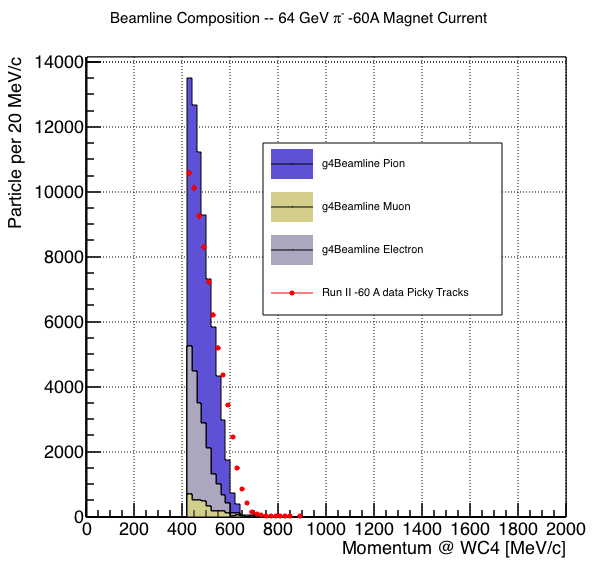
\includegraphics[width=0.5\textwidth,height=\textheight,keepaspectratio]{Chapter-5/Images/Beam60A.png}
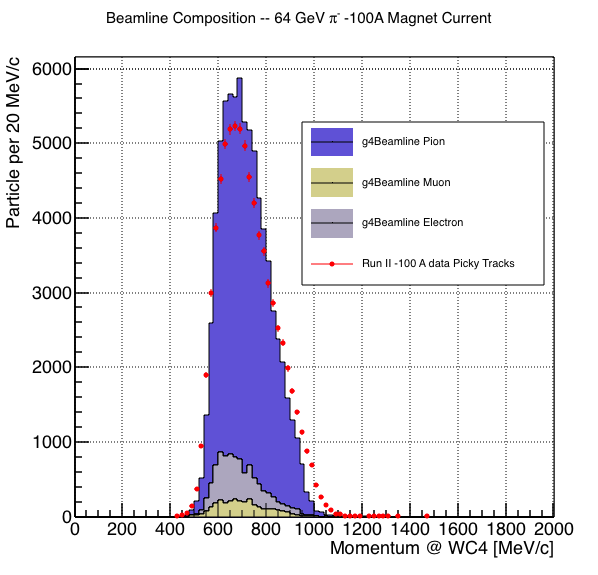
\includegraphics[width=0.5\textwidth,height=\textheight,keepaspectratio]{Chapter-5/Images/Beam100A.png}
\caption{Beam composition for the -60A runs (left) and -100A runs (right). The solid blue plot represents the simulated pion content, the yellow plot represents the simulated muon content and the grey plot represents the simulated electron content. The plots are area normalized to the number of data events, shown in red. }
\label{fig:BeamComposition}
\end{figure}

Table \ref{tab:beamline} shows the beam composition per magnet setting after the mass selection according to the G4Beamline simulation.
\begin{table}[]
\centering
\begin{tabular}{|l|c|c|}
\hline
                     & I = -60 A           & I = -100 A \\ \hline
G4Pions       &   68.8 \%           &      87.4 \%        \\ \hline
G4Muons     &     4.6 \%           &        3.7 \%         \\ \hline
G4Electrons &   26.6 \%           &        8.9 \%        \\ \hline
\end{tabular}
\caption{Simulated beamline composition per magnet settings}
\label{tab:beamline}
\end{table}


\subsubsection{Beam Composition for Positive Kaon Cross Section}
In the positive polarity runs, the tertiary beam composition is mainly pions and protons. The left side of Figure \ref{fig:BeamCompositionPos} shows the  predictions for the momentum spectra for the 100A positive runs  according to  G4Beamline (solid colors) overlaid with data (black points). 
Since the LArIAT beamline detectors can discriminate between kaons and other particles, we do not rely on the G4Beamline simulation to estimate the beamline contamination in the pool of kaon candidates (as in the case of the pion cross section), but rather we use a data drive approach. 
The basic idea of this data driven approach is to estimate the bleed over from high and low mass peaks under the kaon peak by fitting the tails of the $\pi/\mu/e$ and proton mass distributions, as shown in Figure \ref{fig:BeamCompositionPos} right side. 
Since the shape of the tails is unknown, the estimate is done multiple times varying the range and shape for reasonable functions. 
For example, to estimate the proton content under the kaon peak, we start by fitting the left tail of the proton mass distribution with a gaussian function between 650 $MeV/c^2$ and 750 $MeV/c^2$.% in a reasonable range and with a reasonable function. 
We extend the fit function under the kaon peak and integrate the between 350-650 $MeV/c^2$. We integrate the mass histogram in the same range and calculate the proton contamination as the ratio between the two integrals. We repeat this procedure for several fit shapes (gaussian, linear and exponential functions are used) and tail ranges. Finally, we calculate the contamination as the weighted average of single estimates, where the weights are calculated to be the $1./\chi^2$ of the tail fits. The procedure is repeated for lighter particles mass peak independently.
With 12 iterations of this method we find a proton contamination of  0.2 $\pm$ 0.5 \%  and a contamination from the lighter particles of 5 $\pm$ 2 \% .



\begin{figure}
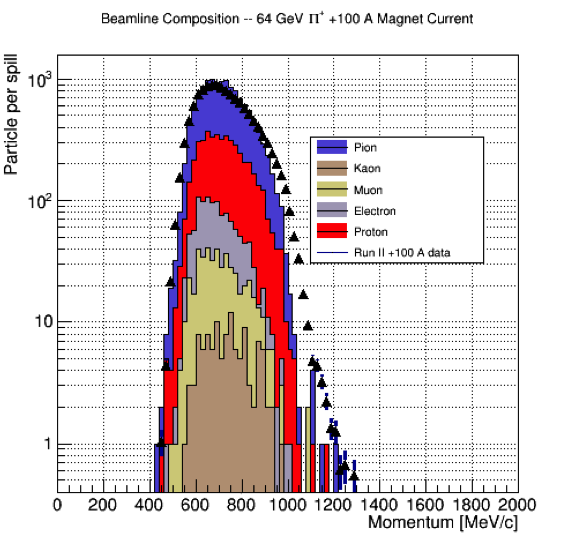
\includegraphics[width=0.5\textwidth,height=\textheight,keepaspectratio]{Chapter-5/Images/Beam100Pos.png}
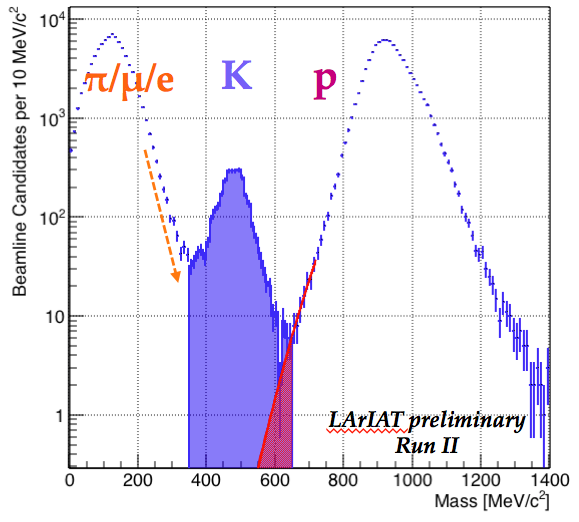
\includegraphics[width=0.5\textwidth,height=\textheight,keepaspectratio]{Chapter-5/Images/MassPos.png}
\caption{$Left.$ Beam composition for the +100A runs after WC4 (no mass selection applied). The solid blue plot represents the simulated pion content, the yellow plot represents the simulated muon content and the grey plot represents the simulated positron content, the red the proton content and the mustard the kaon content. The plots are area normalized to the number of data events, shown in black.$Right.$ Mass distribution for the Run-II positive runs, where the area under the kaon mass peak is highlighted in purple. The area under the extension of a possible fit for the proton tail is highlighted in red. }
\label{fig:BeamCompositionPos}
\end{figure}



\subsection{Data Driven MC}\label{sec:DDMC}
The Data Driven single particle Monte Carlo (DDMC) is a single particle gun which simulates the particle transportation from WC4 into the TPC leveraging on the beamline data information. The DDMC uses the data momentum and position at WC4 to derive the event generation: a general sketch of the DDMC workflow is shown in Figure \ref{fig:DDMCSketch}.

When producing a DDMC sample, beam line data from a particular running period and/or running condition are selected first. For example, data for the negative 60A runs and for the negative 100A runs inform the event generation stage of two different DDMC samples. Figure \ref{fig:DDMCQuantities}  schematically shows the data quantities of interest leveraged from data: the momentum ($P_x, P_y, P_z$) and position ($X, Y$) at WC4. For each data event, we obtain the  particle position ($X, Y$) at WC4 directly from the data measurement; we calculate the components of the momentum using the beamline measurement of the momentum magnitude in conjunction with the hits on WC3 and WC4 to determine the direction of the momentum vector, as described in section \ref{sec:MWPCfunc}. The momentum and position of the selected data form a 5-dimensional tupla, which we sample thousands of times through a 5-dimensional hit-or-miss sampling procedure to generate the MC events. This produces MC $P_x, P_y, P_z, X, Y$ distributions  with the same momentum and position distributions as data, with the additional benefit of accounting for the correlations between the considered variables.  As an example, the results of the DDMC generation compared to data for the kaon +100A sample are shown in figure \ref{fig:DDMCComparison} for the $P_z$, $X$ and $Y$ distributions; as expected, MC and data agree within the statistical uncertainty by construction. A LArSoft simulation module then launches single particle MC from z = -100 cm (the location of the WC4) using the MC generated events. The particles are free to decay and interact in their path from WC4 to the TPC according to the Geant4 simulation.

Using the DDMC technique ensures that the MC and data particles have very similar momentum, position and angular distributions at WC4 and allows us to use the MC sample in several occasions, for example to calibrate the energy loss upstream of the TPC (see Section \ref{ch:eloss}) or to study the tracking and the calorimetric performance (sections \ref{sec:TrackingStudies} and \ref{ch:energyCal}). A small caveat is in order here: the DDMC is a single particle Monte Carlo, which means that the beam pile-up is not simulated. 


Six samples are the basis fo the MC used in the pion cross section measurement: three samples of  $\sim$340000 pions, muons and electrons to simulate the negative 60A runs, and three samples of $\sim$340000 pions, muons and electrons for the negative 100A runs.

The MC used for the kaon cross section analysis is a sample of \textcolor{red}{NUMBERS}  kaons.

\begin{figure}[hpbt]
\centering
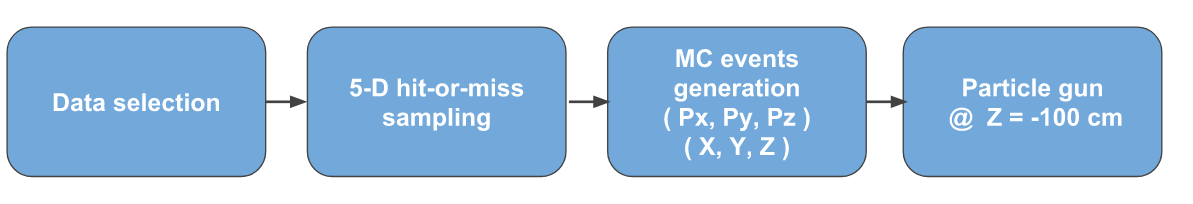
\includegraphics[width=\textwidth]{Chapter-5/Images/DDMCScheme.png}
\caption{Workflow for Data Driven single particle Monte Carlo production.}
\label{fig:DDMCSketch}
\end{figure}


\begin{figure}[hpbt]
\centering
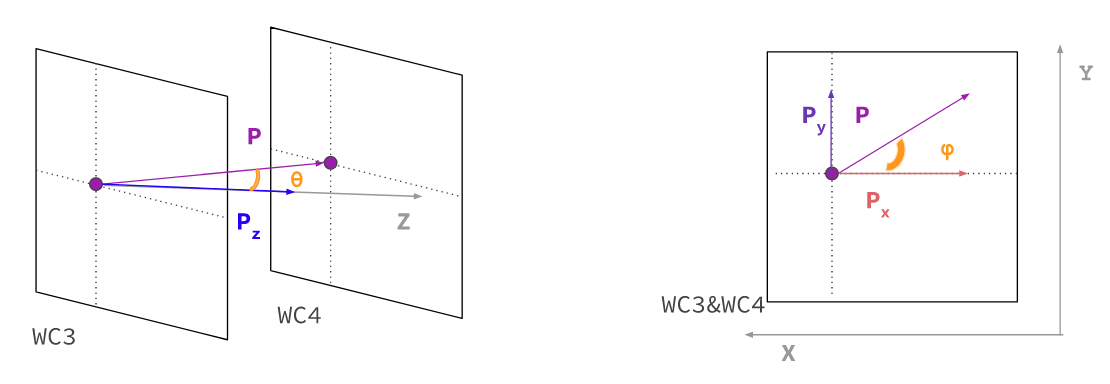
\includegraphics[width=\textwidth]{Chapter-5/Images/DDMCQuantities.png}
\caption{Scheme of the quantities of interest for the DDMC event generation: $P_x, P_y, P_z, X, Y$ at WC4.}
\label{fig:DDMCQuantities}
\end{figure}


\begin{figure}[hpbt]
\centering
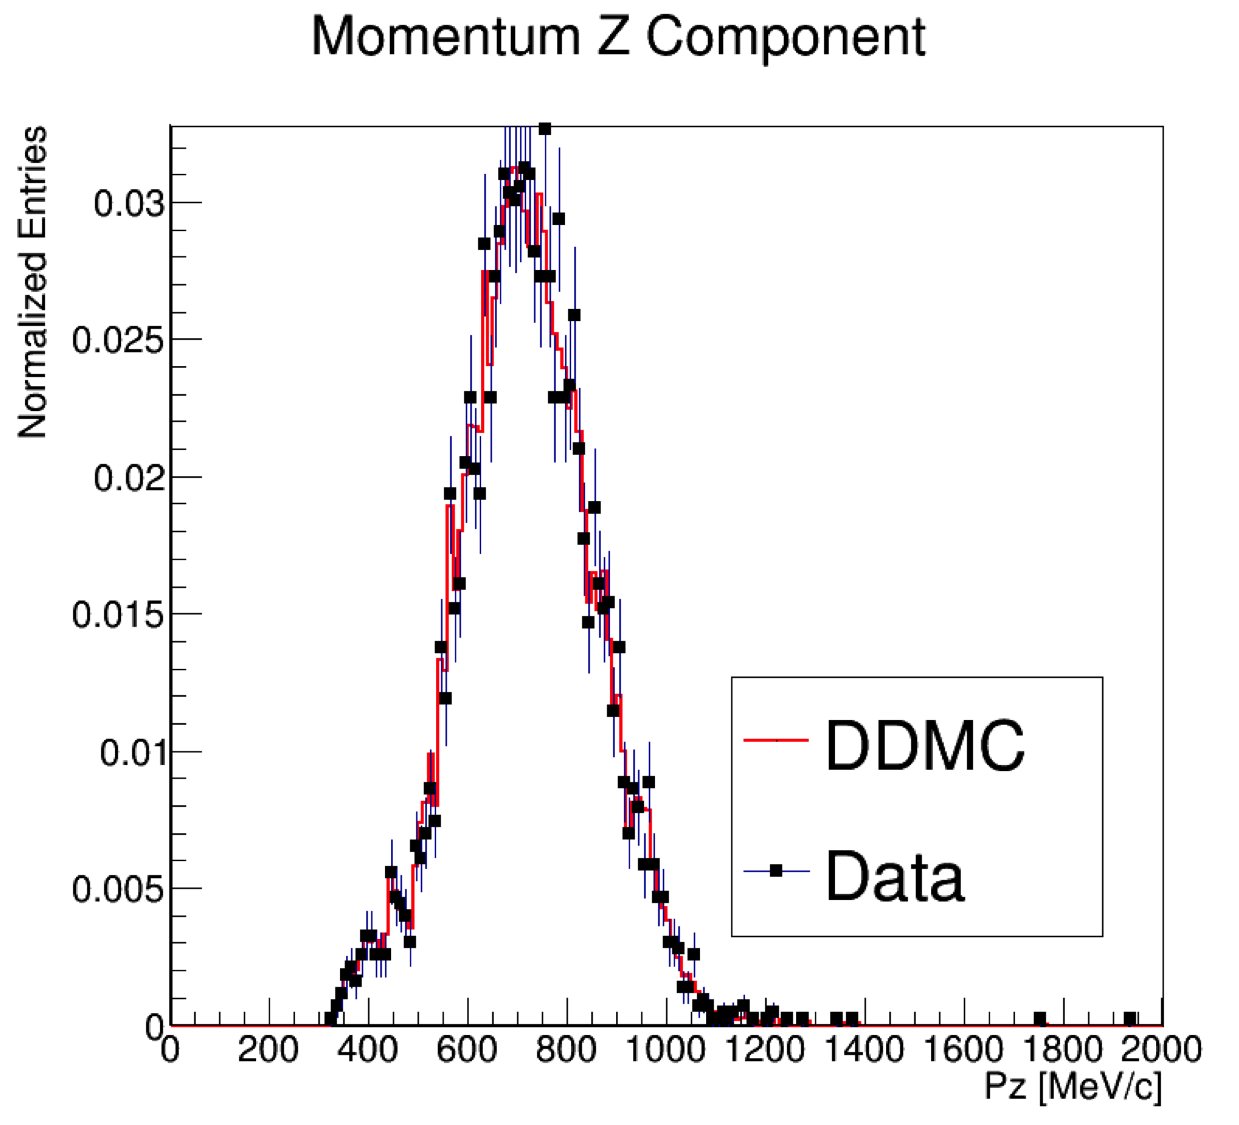
\includegraphics[width=0.48\textwidth]{Chapter-5/Images/DDMCPz.png}
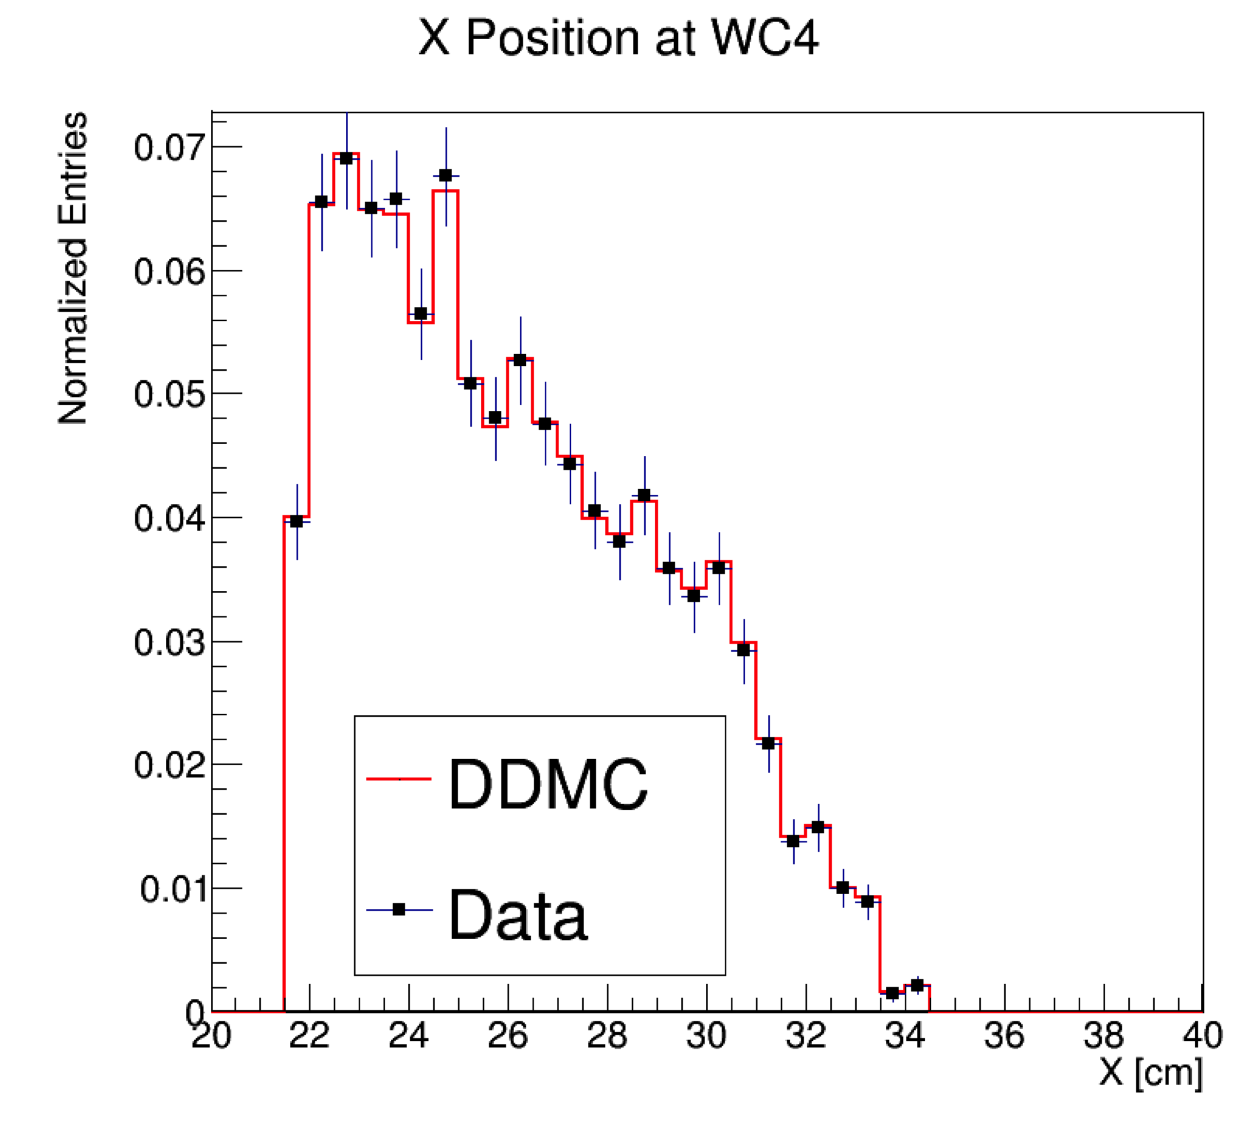
\includegraphics[width=0.48\textwidth]{Chapter-5/Images/DDMCX.png}
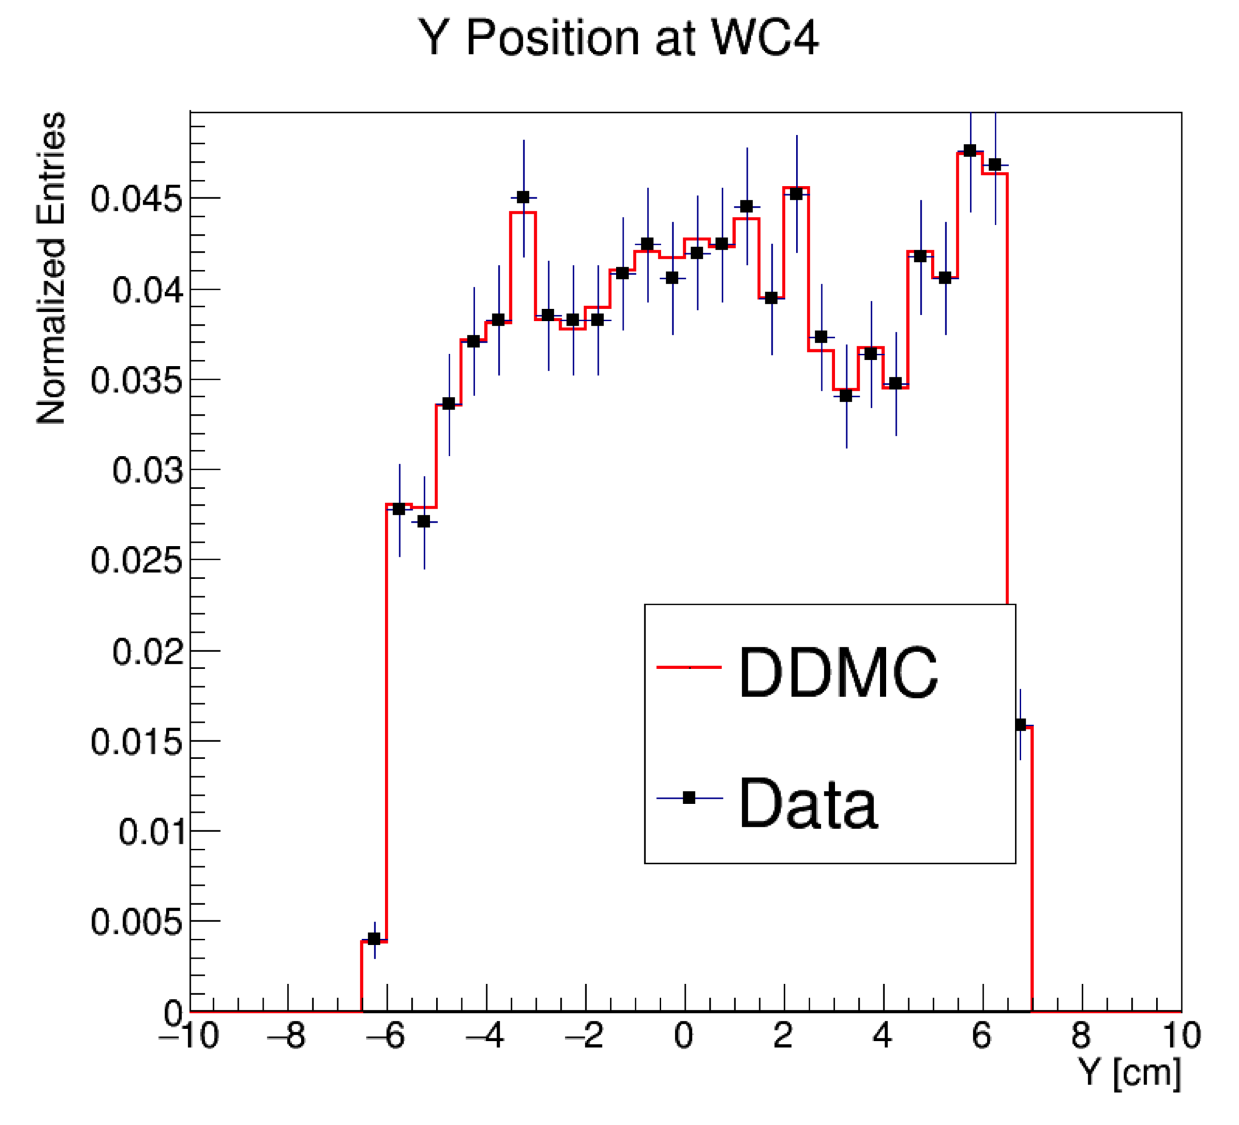
\includegraphics[width=0.48\textwidth]{Chapter-5/Images/DDMCY.png}
\caption{Comparison between generated quantities and data distributions for the 100A kaon sample: Z component of the momentum at WC4 (top left), X position at Wire Chamber 4 (top right), Y position at Wire Chamber 4 (bottom).}
\label{fig:DDMCComparison}
\end{figure}



\subsection{Estimate of Energy Loss before the TPC}\label{ch:eloss}
The beamline particles travel a path from where their  momentum is measured in the beamline until they are tracked again inside the TPC. In the LArIAT geometry, a particle leaving the WC4 will encounter the materials listed in Table \ref{tab:budget} before being registered again. The energy lost by the particle in this non-instrumented material modifies the particle's kinetic energy and directly affects the cross section measurement, as shown in equation \ref{eq:enFF}.

\begin{table}[h!]
\centering
\begin{tabular}{|l|l|l|}
\hline
Material  & density {[}g/cm$^3${]} & width {[}cm{]}    \\ \hline
Fiberglass laminate (G10)      & 1.7                             & 1.28                              \\
Liquid Argon                           & 1.4                             & 3.20                             \\
Stainless Steel                        & 7.7                            & 0.23                             \\
Titanium                                  & 4.5                            & 0.04                             \\ 
Air                                            &  1.2 $\cdot10^{-3}$  & 89.43                              \\
Plastic Scintillator                    & 1.03                          & 1.20 (+ 1.30)                             \\ \hline
\end{tabular}
\caption{LArIAT material budget from WC4 to the TPC Front Face.}
\label{tab:budget}
\end{table}


We derive an estimate of the energy loss between the beamline momentum measurement and the TPC ($E_{loss}$) from the pion DDMC sample, since this quantity is not  measurable directly on data. 
The $E_{loss}$ distribution for the 60A  and 100A pion sample is shown in figure \ref{fig:ELoss60A}, left and right respectively. A clear double peaked structure is visible, which is due to the particles either missing or hitting the HALO paddle: a schematic rendering of this occurrence is  shown in figure \ref{fig:Halo}. The kinematic at WC4 determines the trajectory of a particle and whether or not it will hit the halo paddle. In figure \ref{fig:PxVsXTrue} , we plot the true  horizontal component of the momentum $P_x$ versus the true $X$ position at WC4 for pions missing the halo paddle (left) and for pions hitting the halo paddle (right) for the 60A MC simulation runs -- analogous plots are obtained with the 100A simulation. These distributions can be separated drawing a line in this position-momentum space. 
We use a logistic regression  \cite{agresti2013categorical}  as a classifier to find the best separating line, shown in both plots as the red line. We classify as ``hitting the halo paddle" all pions whose $P_x$ and $X$ are such that $$P_x +0.02* X - 0.4 < 0 $$ and as ``missing the halo  paddle" all pions whose $P_x$ and $X$ are such that $$P_x +0.02*X - 0.4 > 0, $$ where the coefficients of the line are empirically found by the logistic regression estimation. Overall, this simple methode classifies in the right category (hit or miss) about 86\% of the pion events. In MC, we assign  $E_{loss} = 32 \pm 4 $~MeV for pion events classified as ``hitting the halo paddle"; we assign  $E_{loss} = 24 \pm 3 $~MeV for pion events classified as ``missing the halo paddle". We apply the same classifier on data. A scan of the simulated geometry showed an excess of 3 cm of un-instrumented argon compared with the surveyed detector geometry. We account for this difference by assigning in data $E_{loss} = 24 \pm 6 $~MeV for pion events classified as ``hitting the halo paddle" and  $E_{loss} = 17 \pm 6 $~MeV for pion events classified as ``missing the halo paddle", where the uncertainty is derived as the standard deviation of the double peaked distribution.

The summary of the values for used for $E_{Loss}$ for the pion sample is listed in table \ref{tab:Eloss}  with the analogous results for the study on the kaon case.

\begin{table}[b]
\centering
\begin{tabular}{|l|c|c|}  
\hline
                          &  \multicolumn{2}{c|}{E$_{loss}$ [MeV]}    \\ \hline
                          & Hitting Halo          & Missing Halo     \\ \hline
Pion  MC           &  $32 \pm 4 $         &    $24 \pm 3$     \\ \hline
Pion Data          &  $25 \pm 6$          &    $17 \pm 6 $    \\ \hline
Kaon  MC          &  $37 \pm 5 $        &     $31 \pm 4 $    \\ \hline
Kaon Data         &  $26 \pm 6 $        &     $22 \pm 6 $    \\ \hline
\end{tabular}
\caption{Energy loss for pions and kaons.}
\label{tab:Eloss}
\end{table}



%We use the separation of these two distributions to decide what the energy loss for each event on data. 
%Thus,  we assign the value for energy loss is used in the data.


\begin{figure}[hbpt]
\centering
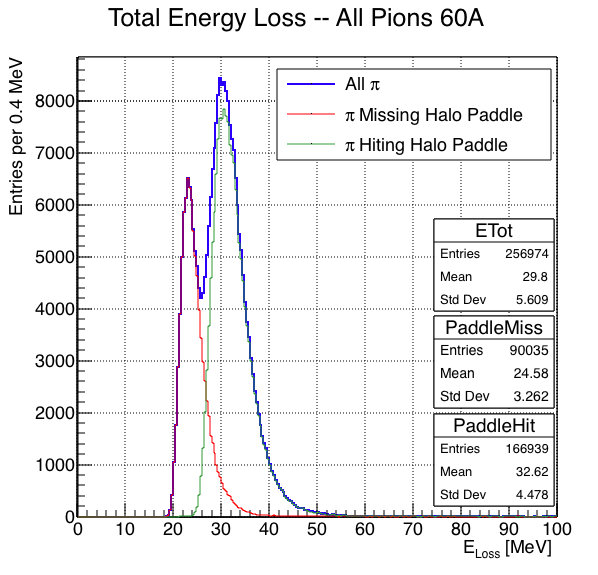
\includegraphics[width=0.45\textwidth]{Chapter-5/Images/E_loss60A.png}
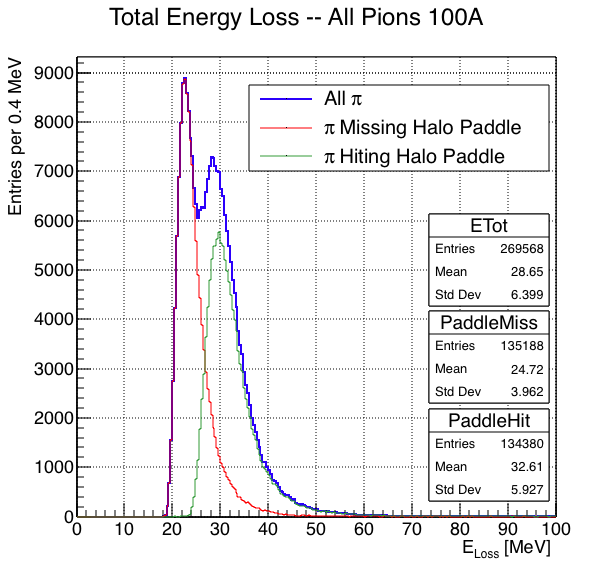
\includegraphics[width=0.45\textwidth]{Chapter-5/Images/E_loss100A.png}
\caption{True energy loss between WC4 and the TPC front face according to the MC simulation of negative pions of the 60A runs (left) and of the 100A runs (right). The distribution for the whole data sample is shown in blue, the distribution for the pions missing the halo is shown in red, and the distribution for the pions hitting the halo is shown in green.  }
\label{fig:ELoss60A}
\end{figure}

\begin{figure}[hbpt]
\centering
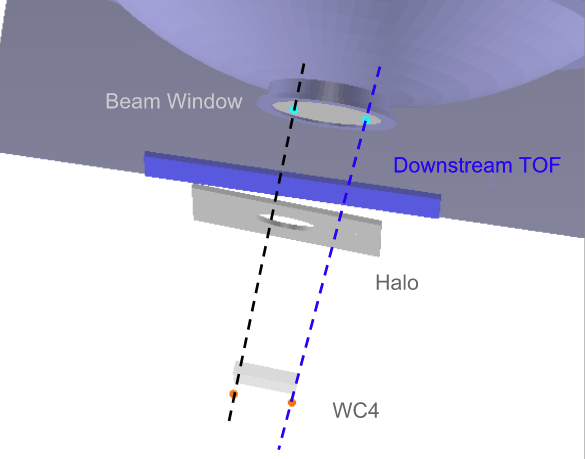
\includegraphics[scale=0.5]{Chapter-5/Images/Halo.png}
\caption{Schematic rendering of the particle path between WC4 and the TPC front face. The paddle with the hollow central circle represents the Halo paddle. We illustrate two possible trajectories: in black, a trajectory that miss the paddle and goes through the hole in the Halo, in blue a trajectory that hits the Halo paddle and goes through the scintillation material.}
\label{fig:Halo}
\end{figure}



\begin{figure}[hbpt]
\centering
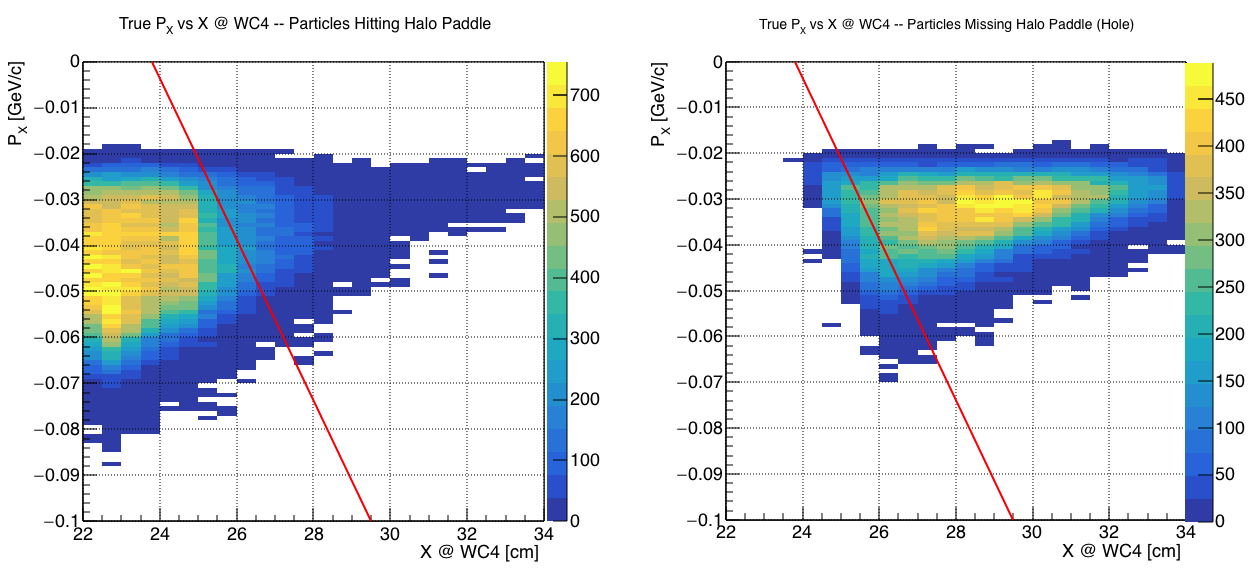
\includegraphics[width=\textwidth]{Chapter-5/Images/PXVsX60A.png}
\caption{Horizontal component of the true momentum vs the horizontal position at WC4 for MC simulated pions of the 60A runs. The plot on the left shows the distribution for pion that miss the halo paddle and the plot on the right shows the distributions for pions that hit the halo. The form of the classifier is overlaid to both plots (red line).}
\label{fig:PxVsXTrue}
\end{figure}



\section{Tracking Studies}\label{sec:TrackingStudies}
In this section, we describe three studies. The first is a justification of the selection criteria for the beamline handshake with the TPC information.  We perform this study to boost  the correct identification of the particles in the TPC associated with the beamline information, while maintaining sufficient statistics for the cross section measurement.  The second study is an optimization of the tracking algorithm, with the scope of maximizing the identification of the hadronic interaction point inside the TPC.  These two studies are related, since the optimization of the tracking is performed on TPC tracks which have been matched to the wire chamber track; in turn, the tracking algorithm for TPC tracks determines the number of reconstructed tracks in each event used to try the matching with the wire chamber track. Starting with a sensible tracking reconstruction, we perform the WC2TPC matching optimization first, then the tracking optimization. The WC2TPC match purity and efficiency  are then calculated again with the optimized tracking.

The third study is an evaluation of  the angular resolution of the tracking algorithm in data and MC, which is particularly important in the context of the cross section analyses.



\subsection{Study of WC to TPC Match}\label{ch:WC2TPCMatchOptimization}

Plots I want in this section:
\begin{enumerate}
\item WC2TPC MC DeltaX, DeltaY and $\alpha$
\end{enumerate}


Scope of this study is assessing the goodness of the wire chamber to TPC match on Monte Carlo and decide the selection values we will use on data. A word of caution is necessary here. With this study, we want to minimize pathologies associated with the presence of the primary hadron itself, e.g. the incorrect association between the beamline hadron and its decay products inside the TPC.  Assessing the contamination from pile-up\footnote{We remind the reader that the DDMC is a single particle Monte Carlo, where the beam pile up is not simulated.}, albeit related, is beyond the scope of this study.

In MC, we are able to define a correct WC2TPC match using the Geant4 truth information. We are thus able to count how many times the WC tracks is associated with the wrong TPC reconstructed track. 

We define a correct match if the all following conditions are met:
\begin{itemize}
\item[-] the length of the true primary Geant4 track in the TPC is greater than 2 cm,  
\item[-] the length of the reconstructed track length is greater than 2 cm,
\item[-] the Z position of the first reconstructed point is within 2 cm from the TPC front face
\item[-] the distance between the reconstructed track and the true entering point is the minimum compared with all the other reconstructed tracks.
\end{itemize}

In order to count the wrong matches, we consider all the reconstructed tracks whose Z position of the first reconstructed point lies within 2 cm from the TPC front face. Events with true length in TPC $<$ 2 cm are included. 
Since hadrons are shot 100 cm upstream from the TPC front face, the following two scenarios are possible from a truth standpoint: 
\begin{itemize}
\item[[$Ta$]] the primary hadron decays or interact strongly before getting to the TPC,
\item[[$Tb$]] the primary hadron enters the TPC.
\end{itemize}

As described in Section \ref{ch:WC2TPCMatchMethod}, we define a WC2TPC match according to the relative position of the WC and TPC track parametrized with $\Delta R$ and the angle between them, parametrized with $\alpha$. Once we choose the selection values $r_{T}$ and $\alpha_{T}$ to determine a reconstructed WC2TPC match, the following five scenarios are possible in the truth to reconstruction interplay : 
\begin{itemize}
\item[1)] only the correct track is matched
\item[2)] only one wrong track is matched 
\item[3)] the correct track and one (or more) wrong tracks are matched
\item[4)] multiple wrong tracks  matched.
\item[5)] no reconstructed tracks are matched
\end{itemize}

Since we keep only events with one and only one match, we discard cases 3), 4) and 5) from the events used in the cross section measurement. For each set of $r_{T}$ and $\alpha_{T}$ selection value, we define purity and efficiency of the selection as follows:
\begin{equation}
\text{Efficiency} = \frac{\text{Number of events correctly matched}}{\text{ Number of events with primary in TPC}},
\end{equation}

\begin{equation}
\text{Purity} = \frac{\text{Number of events correctly matched}}{\text{Total number of matched events}}.
\end{equation}

Figure \ref{fig:EffPurityK} shows the efficiency (left) and purity (right) for WC2TPC match as a function of the radius, $r_{T}$, and angle, $\alpha_{T}$, selection value. It is apparent how both efficiency and purity are fairly flat as a function of the radius selection value at a given angle. This is not surprising. Since we are studying a single particle gun Monte Carlo sample, the wrong matches can occur only for mis-tracking of the primary or for association with decay products;  decay products will tend to be produced at large angles compared to the primary, but could be fairly close to the in $x$ and $y$ projection of the primary. The radius cut would play a key role in removing pile up events. 

For LArIAT cross section measurements, we generally prefer purity over efficiency, since a sample of particles of a pure species will lead to a better measurement. Obviously, purity should be balanced with a sensible efficiency to avoid rejecting the whole sample. 

We choose $(\alpha_{T}$, $r_{T}) = (8 \text{ deg}, 4 \text{ cm} )$ and get a MC 85\% efficiency and 98\% purity for the kaon sample and a MC 95\% efficiency and 90\% purity for the pion sample.


\begin{figure}[hpbt]
\centering
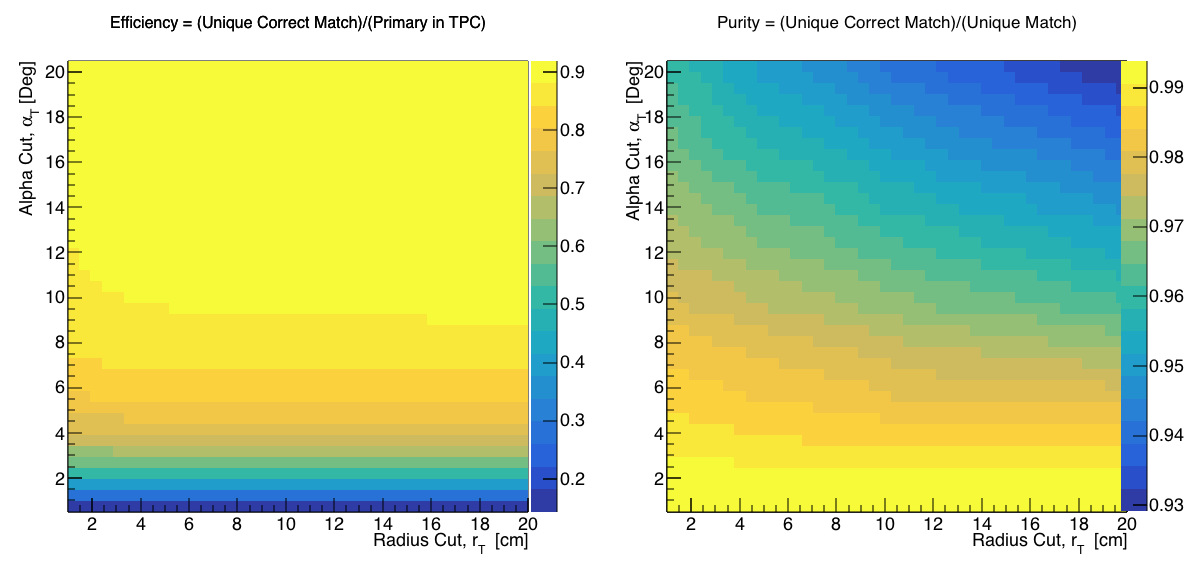
\includegraphics[width=15cm]{Chapter-5/Images/KEffPurity.png}
\caption{Efficiency (left) and purity (right) for WC2TPC match as a function of the radius and angle selections for the kaon sample.}
\label{fig:EffPurityK}
\end{figure}




\subsection{Tracking Optimization}\label{ch:TrackOptimization}


\subsection{Angular Resolution}\label{sec:angleRes}
Scope of this study is to understand and compare the tracking performances and angular resolution of the TPC tracking on data and MC. 
We use the angular resolution of the tracking to determine  the value of smallest angle that we can reconstruct with a non-zero efficiency, effectively determining a selection on the angular distribution of the cross section measurement due to the tracking performance. This study is performed on the pion sample, but its results are extrapolated to the kaon case.

We start by selecting all the WC2TPC matched tracks used for the cross section analysis.  These tracks can contain from a minimum of 3 3D-space points to a maximum of 240  3D-space points.  We fit a line to all the 3D-space points associated with the track. 
For each track we calculate the average distance between each point in space and the fit line as follows 
\begin{equation} 
\bar d = \frac{\sum^N_i d_i}{N},
\end{equation} 
where $N$ is the number of 3D-space points of the track and $d_i$ is the distance of the $i$-th space point to the line fit. Several tests to compare the goodness of fit between data and MC have been considered. We decided to use $\bar d$ for its straightforward interpretation. The $\bar d$ distribution for data and MC is shown in Figure \ref{fig:Chi2AllPts} and shows a relatively good agreement between data and MC.

A visual representation of the procedure used to evaluate the angular resolution is shown in Figure \ref{fig:AngResProcedure}. 
For each track, we order the space points according to their Z position along the positive beam direction (panel a) and we split them in two sets: the first set contains all the points belonging to the first half of the track and the second set contains all the points belonging the second half of the track. We remove the last four points in the first set and the first four points in the second set, so to have a gap in the middle of the original track (panel b). We fit the first and the second set of points with two lines  (panel c). We then calculate the angle between the fit of the first and second half $\alpha$ (panel d). The angle $\alpha$ determines the spatial resolution of the tracking. The distributions for data and MC for $\alpha$ are given in Figure \ref{fig:trackingResolution}. The mean of the data and MC angular resolution are respectively 

\begin{equation}
\bar\alpha_{Data} = (5.0 \pm 4.5) \text{ deg}, 
\end{equation}

\begin{equation}
\bar\alpha_{MC} = (4.5 \pm 3.9) \text{ deg}. 
\end{equation}

Interaction angles smaller than the angle resolution are indistinguishable for the reconstruction. Therefore, we assess our ability to measure the cross section to be limited to interaction angles greater than 5.0 deg. More accurate studies of the angular resolution as a function of the kinetic energy and track length, albeit interesting, are left for an improvement of the analysis. 

It is beneficial to take a moment to describe the definition of interaction angle. In case of elastic scattering, the definition is straightforward: the interaction angle is the angle between the incoming and outgoing pion, i.e.

\begin{equation}  
\theta = \cos^{-1} \Big(\frac{\vec p _{\text{incoming}}  \cdot\vec p _{\text{outgoing}}}{|\vec p _{\text{incoming}}|  |\vec p _{\text{outgoing}}| }\Big).
\end{equation}   
In case of inelastic scattering,  the presence of several topologies requires a more complex definition, as shown in figure \ref{fig:scatterPic}.  We define the scattering angle as the biggest of the angles between the incoming pion and the visible daughters, where the visible daughters are charged particles that travel more than 0.47 cm in the detector (see panel a); in case all the daughters are invisible, the angle is assigned to be 90 deg (see panel b). We chose this working definition of scattering angle for inelastic scattering keeping in mind how our tracking reconstruction works: the tracking will stop correctly in case of all the daughters are not visible in the detector and it is likely to stop correctly if multiple daughters form an interaction vertex. The only ``dangerous" case is the production of one charged daughter plus neutrals, which we can study with this working definition of scattering angle (see panel c).


We can see the effects of the angular resolution on the cross section by plotting the true Geant4 cross section for interaction angles greater than a minimum interaction angle. Figure \ref{fig:trueWithAngles} shows the  true Geant4 cross section  for interaction angles greater than 0 deg (green), 4.5 deg (red), 5.0 deg  (blue) and 9.0 deg (yellow). 
A small $0.5 \text{ deg}$ systematic shift between the mean of the data and MC angular resolution is present.%, which we account for in the context of the MC efficiency correction to the cross section, as presented in \ref{sec:angSys}.

\begin{figure}[ht]
\begin{minipage}[t]{0.45\linewidth}
\centering
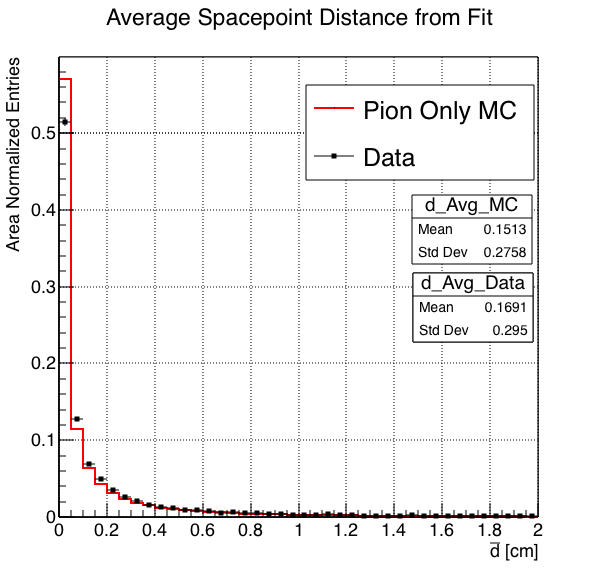
\includegraphics[width=\textwidth]{Chapter-5/Images/cDAvg.png}
\caption[]{Distributions of the average distance between each 3D point in space and the fit line,  $\bar d$ for the data used in the pion cross section analysis and the pion only DDMC. The distributions are area normalized. } \label{fig:Chi2AllPts}
\end{minipage}
\hspace{0.5cm}
\begin{minipage}[t]{0.45\linewidth}
\centering
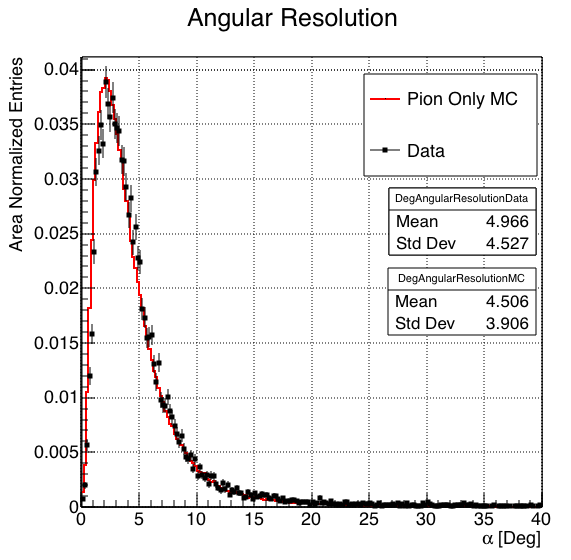
\includegraphics[width=\textwidth]{Chapter-5/Images/cTrackingDeg.png}
\caption[]{Distributions of angular resolution $\alpha$ for data used in the pion cross section analysis and pion only DDMC. The distributions are area normalized. } \label{fig:trackingResolution}
\end{minipage}
\end{figure}




\begin{figure}[ht]
\begin{minipage}[t]{0.45\linewidth}
\centering
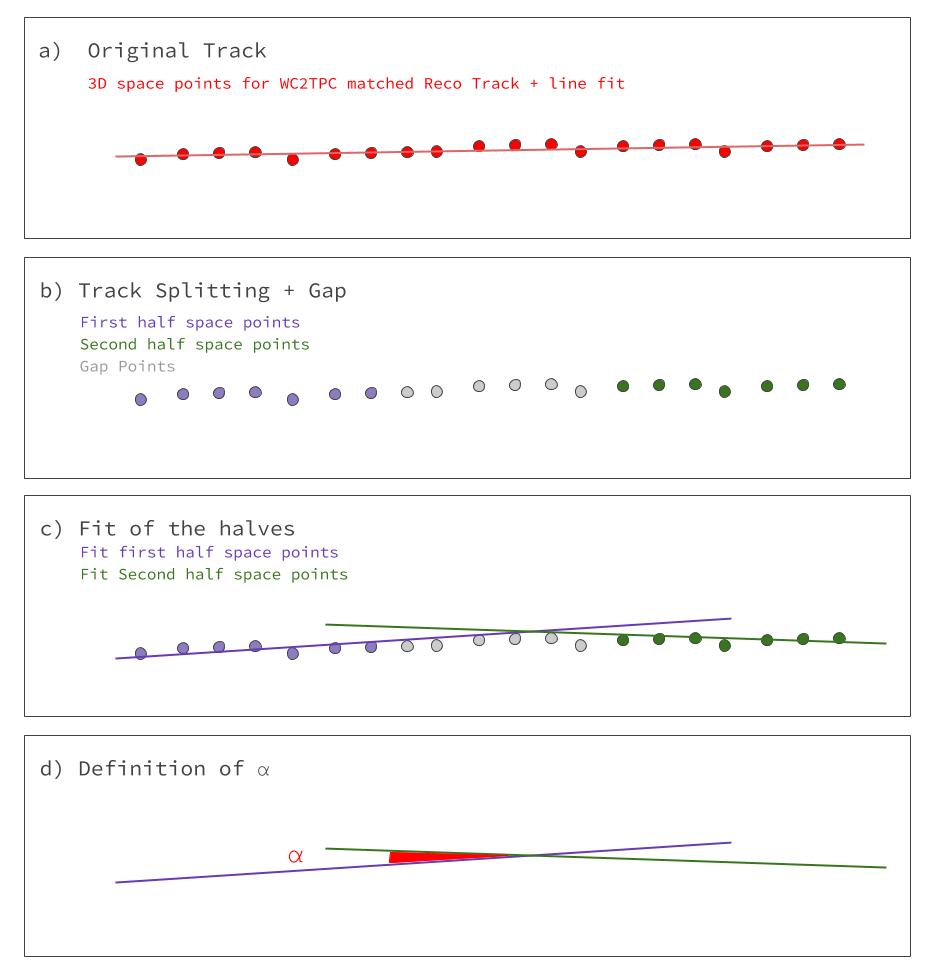
\includegraphics[width=\textwidth]{Chapter-5/Images/TrackingProcedure.png}
\caption{A visual representation of the procedure used to evaluate the angular resolution.}
\label{fig:AngResProcedure}
\end{minipage}
\hspace{0.5cm}
\begin{minipage}[t]{0.45\linewidth}
\centering
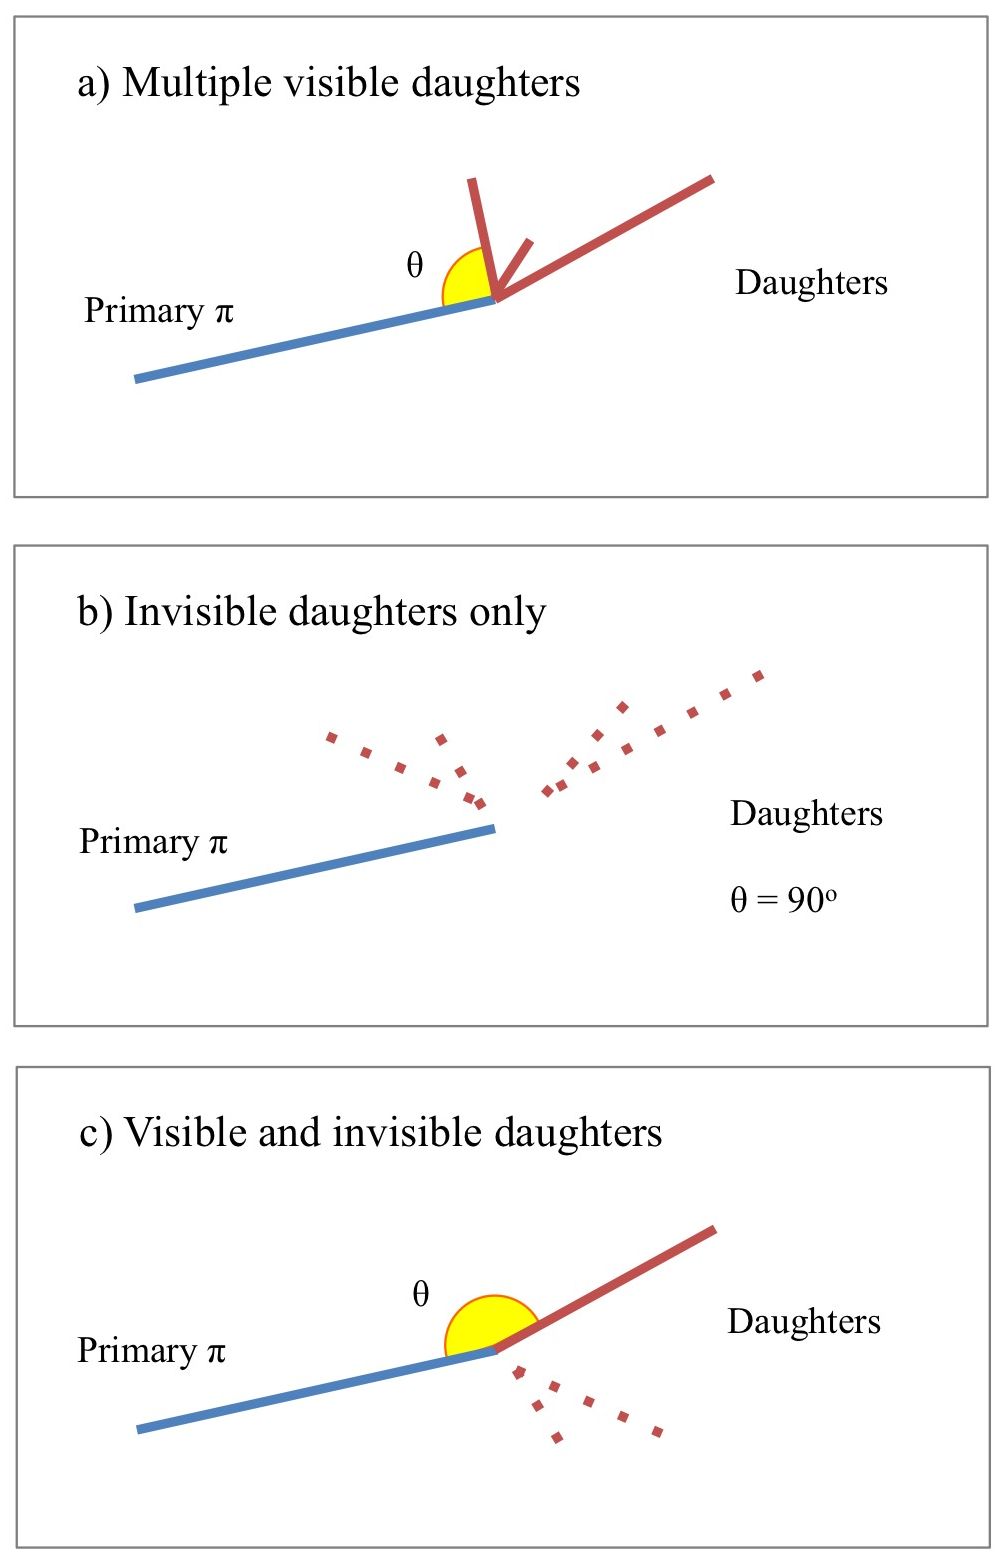
\includegraphics[width=\textwidth]{Chapter-5/Images/Daughters.png}
\caption{A visual representation of the scattering angle definition in case of inelastic scattering.}
\label{fig:scatterPic}
\end{minipage}
\end{figure}

\begin{figure}[p]
\centering
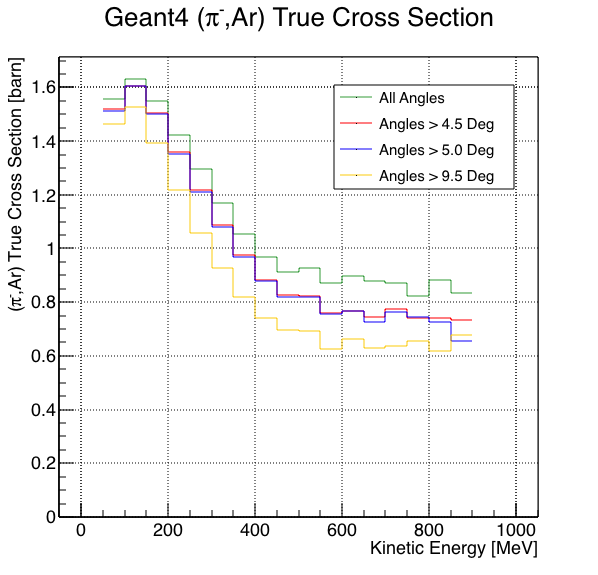
\includegraphics[width=0.48\textwidth]{Chapter-5/Images/cTrueXSAngle.png}
\caption{ True ($\pi^-, Ar$) cross section for interaction angles greater than 0 deg (green), 4.5 deg (red), 5.0 deg  (blue) and 9.0 deg (yellow). }
\label{fig:trueWithAngles}
\end{figure}



\clearpage
%%%%%%%%%%%%%%%%%%%%%%%%%%%%%%%%%%%%%%%%%%%%%%%%%%%%%%%%%%%%%%
%%%%%%%%%%%%%%%%%%%%%%%%%%%%%%%%%%%%%%%%%%%%%%%%%%%%%%%%%%%%%%
%%%%%%%%%%%%%%%%%%%%%%%%%%%%%%%%%%%%%%%%%%%%%%%%%%%%%%%%%%%%%%

\section{Calorimetry Studies}\label{ch:energyCal} 
The ability to measure the kinetic energy of hadrons in the TPC is fundamental for the cross section analyses. 
Thus, we describe first how we calibrate the TPC calorimetric response (Section \ref{ch:energyCalibration}) and how we measure the kinetic energy of the hadrons in the TPC (Section \ref{ch:kinEn}).

\subsection{Energy Calibration}\label{ch:energyCalibration}
Scope of the energy calibration is to identify the factors which convert the charge collected (dQ) to energy deposited in the chamber (dE). As described in section \ref{sec:SignalProc}, this is a multi-step procedure. In LArIAT, we first correct the raw charge by the electronic noise on the considered wire \cite{LArIATdqdx}, then by the electron lifetime \cite{LArIATLifeTime},  and then by the recombination using the ArgoNeut recombination values. Lastly, we apply overall calibration of the energy, i.e. we determine the ``calorimetry constants" using the procedure described in this section.


We independently determine  the calorimetry constants for Data and Monte Carlo in the LArIAT Run-II Data samples using  a parametrization of the stopping power (a.k.a. energy deposited per unit length, $dE/dX$)  as a function of momentum. This is done by comparing the stopping power measured on reconstructed quantities against the Bethe-Bloch theoretical prediction for various particle species (see Equation \ref{eq:BB}).  We obtain the theoretical expectation for the $dE/dX$ most probable value of pions ($\pi$), muons ($\mu$), kaons ($K$), and protons ($p$) in the momentum range most relevant for LArIAT (Figure \ref{fig:PDGEnergyLossArgon}) using the tables provided by the Particle Data Group \cite{Patrignani:2016xqp} for liquid argon \cite{PDG-Argon}.

The basic idea of this calibration technique is to utilize a sample of beamline events with known particle species and momentum to measure the $dE/dX$ of the corresponding tracks in the TPC. In particular, we decided to use positive pions as calibration sample and all the other particle species as cross check. Once the $dE/dX$ of a sample of positive pions  has been measured at various momenta, we tune to calorimetry constants within the reconstruction software to align the measured values to match the theoretical ones found in Figure \ref{fig:PDGEnergyLossArgon}. 

In data, we start by selecting a sample of beamline positive pion beamline candidates without any restriction on their measured momentum\footnote{it should be noted that some muon and position contamination is present in the $\pi^+$ sample}.
We then apply the WC2TPC match and subtract the energy loss upstream to the TPC front face, determining the momentum at the TPC front face. For each surviving pion candidate,  we measure the $dE/dx$ at each of the first 12 spacepoints associated the 3D reconstructed track, corresponding to a $\sim$ 5 cm portion. These $dE/dX$ measurements are then put into a histogram that corresponds to measured momentum of the track. The $dE/dX$ histograms are sampled every 50 MeV/c in momentum (e.g. 150~MeV/c $< P <$ 200~MeV/c, 200~MeV/c $< P <$ 250/c~MeV, etc...).   This process of selecting, sampling, and recording the $dE/dX$ for various momentum bins is repeated over the entire sample of events, allowing us to collect sufficient statistic in most of the momentum bins between 150~MeV/c and 1100~MeV/c. On average, pions and muons only lose $\sim$10 MeV in this 5~cm section of the track and protons lose $\sim$20 MeV. Thus choosing 50 MeV/c size bins for our histograms covers the energy spread within those bins due to energy loss from ionization for all the particle species identifiable in the beamline. 
Each 50 MeV/c momentum binned $dE/dX$ histogram is now fit with a simple Landau function. The most probable value (MPV) and the associated error on the MPV from the fit are extracted and plotted against the theoretical prediction Figure \ref{fig:PDGEnergyLossArgon}. Depending on the outcome of the fit, we modify the calorimetry constants and we repeat the procedure until a qualitative agreement is achieved.  We perform this  tuning for the collection and induction plane separately. 
As a cross check to the calorimetry constants determined using the positive pions, we lock the constants and  plot the $dE/dx$ versus momentum distribution of all the other particle species identifiable in the beamline data ($\pi/\mu/e$, K , p, in both polarities) against the corresponding Beth-Bloch prediction. The agreement between data from the other particle species and the predictions is the expected result of this cross check.
The results of the tuning and cross check for Run-II data on the collection plane is shown in Figure \ref{fig:BBandData}  negative polarity data on top, positive polarity data on the bottom.

In MC, we simulate the corresponding positive pion sample with the DDMC (see section \ref{sec:DDMC}) and follow the same steps as in data. More details on the calorimetry tuning can be found in \cite{LArIATCalo}.

\textcolor{red}{Add agreement between data and MC for dedx for pions}

\begin{figure}[htb]
\centering
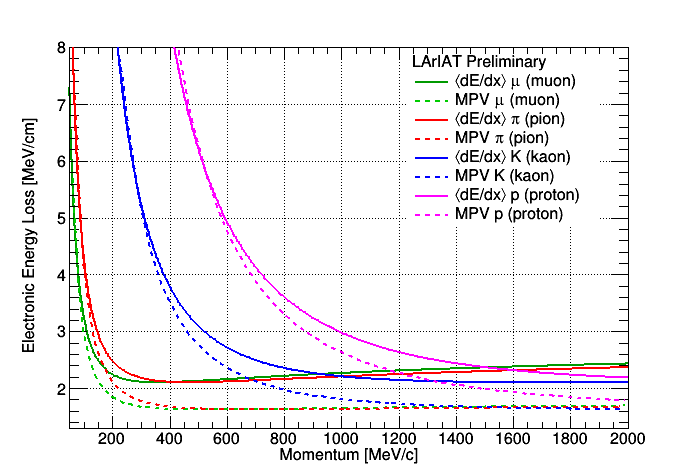
\includegraphics[width=0.50\textwidth]{Chapter-5/Images/dEdXvsMomentumTemplate.png}
\caption{Stopping power for pions, muons, kaons, and protons in liquid argon over the momentum range most relvant for LArIAT according to the Beth-Bloch equation. The solid lines represent the prediction for the mean energy $dE/dX$, while the dashed lines are the predictions for the MPV.}
\label{fig:PDGEnergyLossArgon}
\end{figure}


\begin{figure}[htb]
\centering
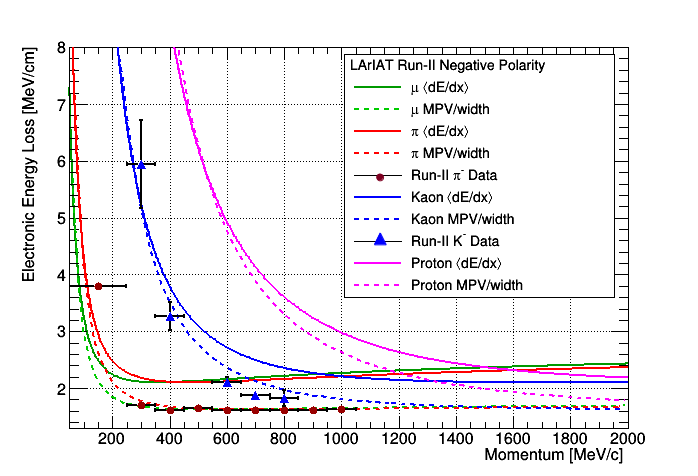
\includegraphics[width=0.50\textwidth]{Chapter-5/Images/RunIINegTotaldEdXvsMomentum.png}
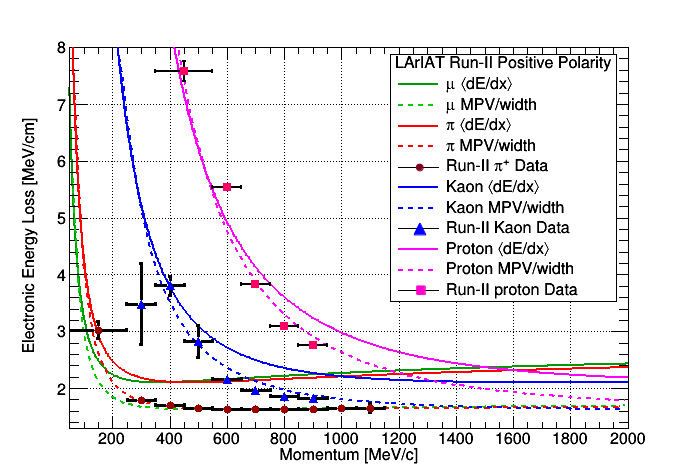
\includegraphics[width=0.50\textwidth]{Chapter-5/Images/RunIIPosTotaldEdXvsMomentum.png}
\caption{Stopping power versus Momentum for Run-II negative (top) and positive (bottom) polarity data. We achieve the agreement between the Bethe-Bloch predictions and the distribution obtained with of the positive pions (top plot, red dots) by tuning the calorimetry constants. Once the calorimetry constants are locked in, the agreement between the other particle species and the Bethe-Bloch predictions follows naturally.}
\label{fig:BBandData}
\end{figure}


%\begin{figure}[htb]
%\centering
%\includegraphics[width=0.50\textwidth]{images/CalibrationExample.png}
%\caption{Illustration of the calibration technique. Here we depict a 325 MeV wire chamber track (shown in green) which enters the TPC (taking into account the energy loss from the upstream material) and we sample the first 12 spacepoints (shown in teal) to extract the dE/dX distribution which is fit with a Landau.}
%\label{fig:CalibrationExample}
%\end{figure}






\subsection{Kinetic Energy Measurement}\label{ch:kinEn}
The measured kinetic energy of a hadron candidate at each argon slab determines which bins of the interacting and incident histograms a selected event is going to fill. In this section, we define the measurement on the kinetic energy and  determine the related uncertainty. We will propagate this uncertainty into the cross section measurement, as discussed in Section \ref{ch:SysUncertaintyXSRaw} for the pion cross section and in Section \ref{ch:SysUncertaintyXSRawKaon} for the kaon cross section.

The kinetic energy of a hadron at the $j^{\text{th}}$ slice of argon in the TPC is given by

\begin{equation}
KE_{j} = \sqrt{p_{Beam}^2 + m_{Beam}^2} - m_{Beam}^2 - E_{Loss} - E_{\text{FF-j}},
\end{equation}

where $p_{Beam}$ is the momentum measured by the beamline detectors,  $m_{Beam}$ is the mass of the hadron as reported in the PDG,  $E_{Loss}$  is the energy loss between the beamline and the TPC, and $ E_{\text{FF-j}}$ is the energy that the hadron deposited from the TPC front face until the $j^{\text{th}}$ slice.
The uncertainty on $KE_{j}$ is then given by 
\begin{equation}
\delta KE_{j} = \sqrt{\delta p_{Beam}^2 + \delta E_{Loss}^2 +  \delta  E_{\text{dep FF-j}}^2},
\end{equation}

where we have dropped the uncertainty on the mass, since it is orders of magnitude smaller than the other uncertainties.
We assume the relative uncertainty on $p_{Beam}$ to be 2\%, and the uncertainty on the energy loss upstream to be 7~MeV, as calculated in Section \ref{ch:eloss}. We describe the estimate of the uncertainty on $E_{\text{FF-j}}$ in the rest of this section.

The energy deposited by the hadron from the TPC front face until the $j^{\text{th}}$ slice is the sum of the measured energy deposited in each previous slabs $E_{i}$, i.e.
\begin{equation}
E_{\text{FF-j}} = \sum_{i<j} E_{i}, 
\end{equation}
where $E_{i}$ is measured in each slab as  the product of the stopping power,  $dE/dX_{i}$,  and the track pitch, $Pitch_i$, for that point. 
If we assume conservatively that the measurements of $E_{i}$ are not independent from one another, the uncertainty on $E_{\text{FF-j}}$ becomes
\begin{equation}
\delta E_{\text{FF-j}} = (j-1) \delta E_{i}, 
\end{equation}
where $\delta E_{i}$ is the uncertainty on the energy loss in one slab of argon.

The left side of Figure \ref{fig:EnergyDeposited} shows the distribution of the energy deposited in each slab of argon, for the 60A negative pion dataset in black and for the pion only MC in blue. The analogous plot for the -100A negative pion data set  is show on the right side of Figure \ref{fig:EnergyDeposited}.  The distributions are fitted with a landau displayed in red for data and in teal for MC.
The uncertainty on $E_{i}$ is given by the width of the Landau fit to the data. A small systematic uncertainty  is given by a 1.0\% difference between the most probable value of the landau fits in data and MC.

\begin{figure}[htb]
\centering
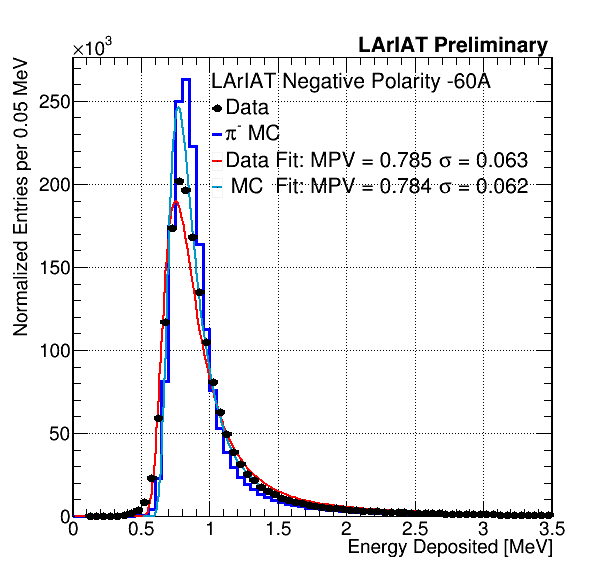
\includegraphics[width=0.48\textwidth]{Chapter-5/Images/DepEnergy_Fit_v4.png}
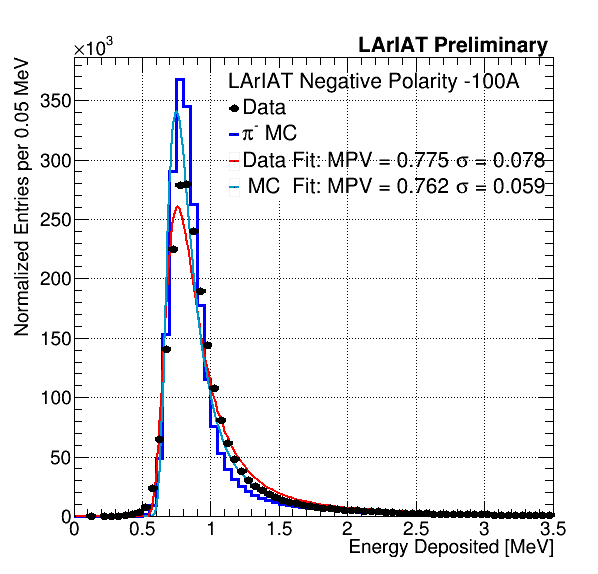
\includegraphics[width=0.48\textwidth]{Chapter-5/Images/DepEnergy_Fit_v4100A.png}
\caption[]{ Energy deposited  $E_{i}$ in a single slab of argon for the pion -60A runs (left) and -100A runs (right).  The data is shown in black, the MC in blue. The distributions are fitted with a landau displayed in red for data and in teal for MC. } \label{fig:EnergyDeposited}
\end{figure}


\begin{comment}

Figure \ref{fig:EnergyDepositedStacked} shows the stacked version of the Energy Deposited plots with the backgrounds stacked. The backgrounds are given in the ratio of 68.8\% pion, 4.6\% muon, and 26.6\% electron. Once they are taken in these ratios, the sum of the MC is normalized to the sum of the data.

\begin{figure}[htb]
\centering
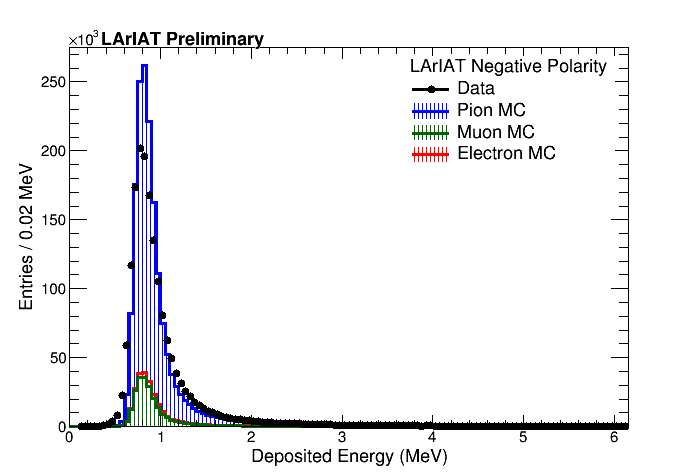
\includegraphics[width=0.48\textwidth]{Chapter-5/Images/DepEnergy_Stacked_v1.png}
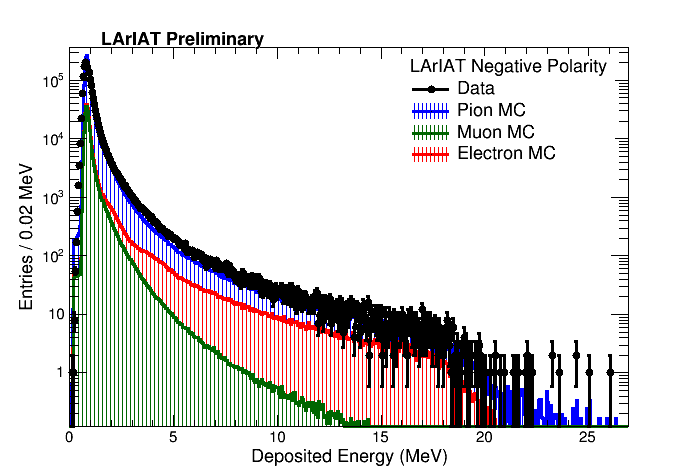
\includegraphics[width=0.48\textwidth]{Chapter-5/Images/DepEnergy_Stacked_v3.png}
\caption[]{ Energy Deposited with all the MC and 60A data.  } \label{fig:EnergyDepositedStacked}
\end{figure}

The energy at the interacting point is given by
\begin{equation}
KE_{Interaction} = \sqrt{P_{WCtrk}^2 + m_{\pi}^2} - E_{Loss} - (\Sigma dE/dX_{i} \times Pitch)
\end{equation}

and has the exact same uncertainty as the incident kinetic energy plot. Thus these estimates can be applied to getting the uncertainty on the energy of the reconstructed cross-section.




%%%%%%%%%%%%%%%%%%%%%%%%%%%%%%%%%%%%%%%%%%%%%%%
\subsection{dE/dX}
%%%%%%%%%%%%%%%%%%%%%%%%%%%%%%%%%%%%%%%%%%%%%%%
Figure \ref{fig:dEdXLinearScale} shows the output of the fit of the Pion MC and the 60 Amp data. The MC is normalized to the data and both are fit to a Landau function. \footnote{The entries at dE/dX = 0 come from an uninitialized variable and can/should be taken out of these plots}

\begin{figure}[htb]
\centering
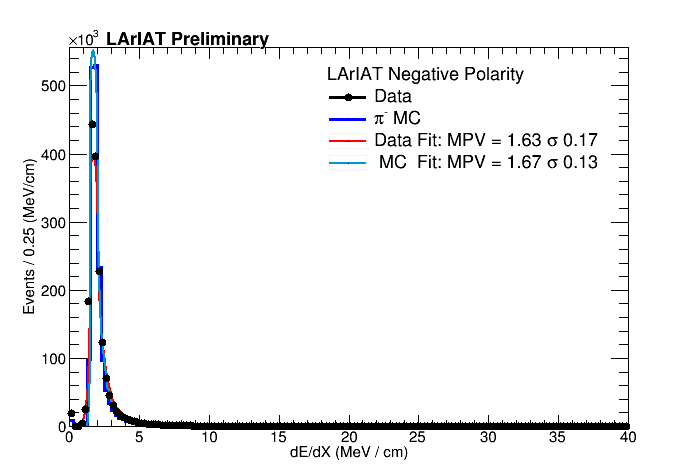
\includegraphics[width=0.48\textwidth]{Chapter-5/Images/dEdX_Fit_v1.png}
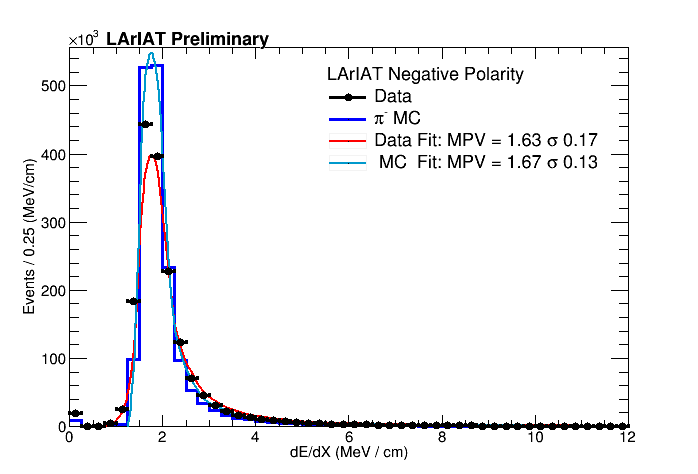
\includegraphics[width=0.48\textwidth]{Chapter-5/Images/dEdX_Fit_v4.png}
\caption[]{ dE/dX for 60Amp data and data driven pion MC, both fit with a Landau  } \label{fig:dEdXLinearScale}
\end{figure}

The difference between the two MPV's, is 2.4\% between the data and the MC.

Figure \ref{fig:dEdXLinearStacked} shows the stacked version of the dE/dX with the backgrounds stacked. The backgrounds are given in the ratio of 68.8\% pion, 4.6\% muon, and 26.6\% electron. Once they are taken in these ratios, the sum of the MC is normalized to the sum of the data.

\begin{figure}[htb]
\centering
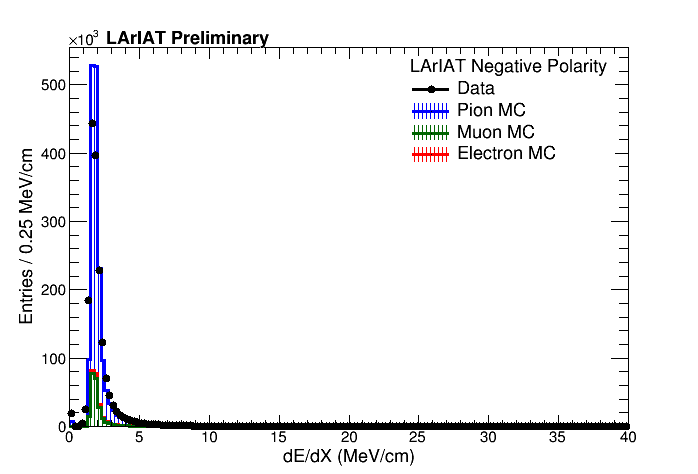
\includegraphics[width=0.48\textwidth]{Chapter-5/Images/dEdX_stacked_v1.png}
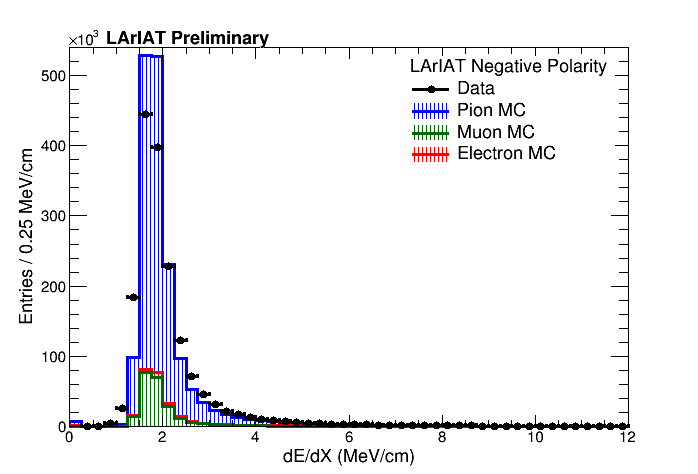
\includegraphics[width=0.48\textwidth]{Chapter-5/Images/dEdX_stacked_v4.png}
\caption[]{ Stacked versions of the dE/dX with the data and electron/muon/pion MC.  } \label{fig:dEdXLinearStacked}
\end{figure}

For completeness, the log scale versions of are shown in Figure \ref{fig:dEdXLogScale}.

\begin{figure}[htb]
\centering
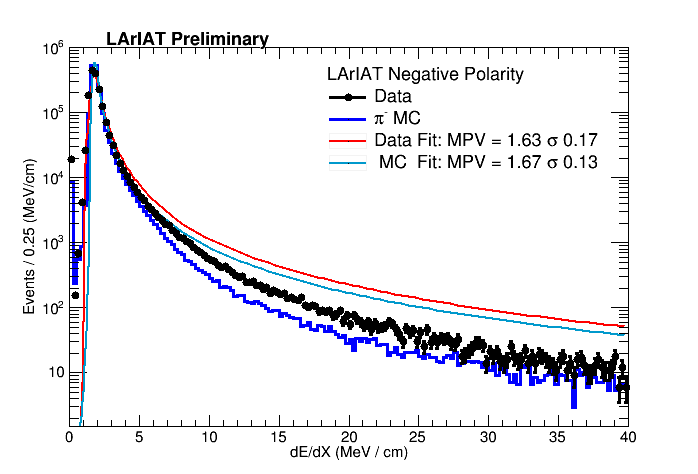
\includegraphics[width=0.48\textwidth]{Chapter-5/Images/dEdX_Fit_v2.png}
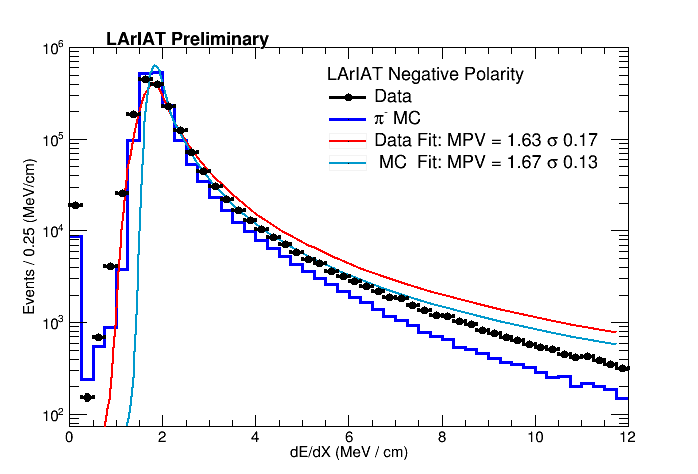
\includegraphics[width=0.48\textwidth]{Chapter-5/Images/dEdX_Fit_v3.png}
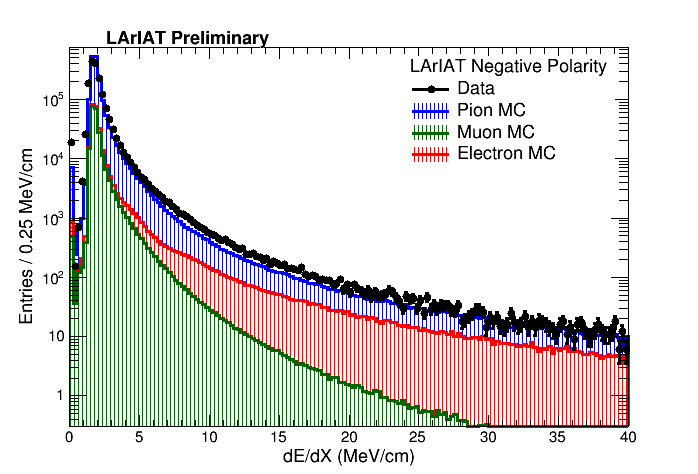
\includegraphics[width=0.48\textwidth]{Chapter-5/Images/dEdX_stacked_v2.png}
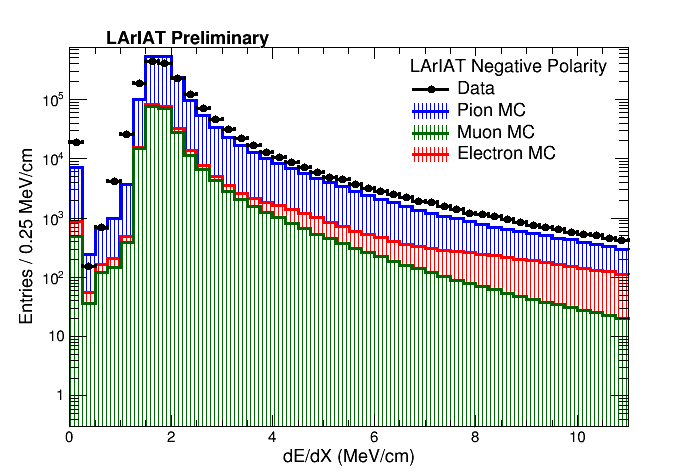
\includegraphics[width=0.48\textwidth]{Chapter-5/Images/dEdX_stacked_v3.png}
\caption[]{ dE/dX for 60Amp data and MC shown in log scale  } \label{fig:dEdXLogScale}
\end{figure}



%%%%%%%%%%%%%%%%%%%%%%%%%%%%%%%%%%%%%%%%%%%%%%%
\subsection{Energy Deposited}\label{sec:Energy}
%%%%%%%%%%%%%%%%%%%%%%%%%%%%%%%%%%%%%%%%%%%%%%%




\end{comment}




